%\documentclass[
  bibliography=totoc,     % Literatur im Inhaltsverzeichnis
  captions=tableheading,  % Tabellenüberschriften
  titlepage=firstiscover, % Titelseite ist Deckblatt
]{scrartcl}

% Paket float verbessern
\usepackage{scrhack}

% Warnung, falls nochmal kompiliert werden muss
\usepackage[aux]{rerunfilecheck}

% unverzichtbare Mathe-Befehle
\usepackage{amsmath}
% viele Mathe-Symbole
\usepackage{amssymb}
% Erweiterungen für amsmath
\usepackage{mathtools}

% Fonteinstellungen
\usepackage{fontspec}
% Latin Modern Fonts werden automatisch geladen
% Alternativ zum Beispiel:
%\setromanfont{Libertinus Serif}
%\setsansfont{Libertinus Sans}
%\setmonofont{Libertinus Mono}

% Wenn man andere Schriftarten gesetzt hat,
% sollte man das Seiten-Layout neu berechnen lassen
\recalctypearea{}

% deutsche Spracheinstellungen
\usepackage[ngerman]{babel}


\usepackage[
  math-style=ISO,    % ┐
  bold-style=ISO,    % │
  sans-style=italic, % │ ISO-Standard folgen
  nabla=upright,     % │
  partial=upright,   % │
  mathrm=sym,        % ┘
  warnings-off={           % ┐
    mathtools-colon,       % │ unnötige Warnungen ausschalten
    mathtools-overbracket, % │
  },                       % ┘
]{unicode-math}

% traditionelle Fonts für Mathematik
\setmathfont{Latin Modern Math}
% Alternativ zum Beispiel:
%\setmathfont{Libertinus Math}

\setmathfont{XITS Math}[range={scr, bfscr}]
\setmathfont{XITS Math}[range={cal, bfcal}, StylisticSet=1]

% Zahlen und Einheiten
\usepackage[
  locale=DE,                   % deutsche Einstellungen
  separate-uncertainty=true,   % immer Unsicherheit mit \pm
  per-mode=symbol-or-fraction, % / in inline math, fraction in display math
]{siunitx}

% chemische Formeln
\usepackage[
  version=4,
  math-greek=default, % ┐ mit unicode-math zusammenarbeiten
  text-greek=default, % ┘
]{mhchem}

% richtige Anführungszeichen
\usepackage[autostyle]{csquotes}

% schöne Brüche im Text
\usepackage{xfrac}

% Standardplatzierung für Floats einstellen
\usepackage{float}
\floatplacement{figure}{htbp}
\floatplacement{table}{htbp}

% Floats innerhalb einer Section halten
\usepackage[
  section, % Floats innerhalb der Section halten
  below,   % unterhalb der Section aber auf der selben Seite ist ok
]{placeins}

% Seite drehen für breite Tabellen: landscape Umgebung
\usepackage{pdflscape}

% Captions schöner machen.
\usepackage[
  labelfont=bf,        % Tabelle x: Abbildung y: ist jetzt fett
  font=small,          % Schrift etwas kleiner als Dokument
  width=0.9\textwidth, % maximale Breite einer Caption schmaler
]{caption}
% subfigure, subtable, subref
\usepackage{subcaption}

% Grafiken können eingebunden werden
\usepackage{graphicx}

% schöne Tabellen
\usepackage{tabularray}
\UseTblrLibrary{booktabs, siunitx}

% Verbesserungen am Schriftbild
\usepackage{microtype}

% Literaturverzeichnis
\usepackage[
  backend=biber,
]{biblatex}
% Quellendatenbank
\addbibresource{lit.bib}
\addbibresource{programme.bib}

% Hyperlinks im Dokument
\usepackage[
  german,
  unicode,        % Unicode in PDF-Attributen erlauben
  pdfusetitle,    % Titel, Autoren und Datum als PDF-Attribute
  pdfcreator={},  % ┐ PDF-Attribute säubern
  pdfproducer={}, % ┘
]{hyperref}
% erweiterte Bookmarks im PDF
\usepackage{bookmark}

% Trennung von Wörtern mit Strichen
\usepackage[shortcuts]{extdash}

\author{%
  Vincent Wirsdörfer\\%
  \href{mailto:vincent.wirsdoerfer@udo.edu}{authorA@udo.edu}%
  \and%
  Joris Daus\\%
  \href{mailto:joris.daus@udo.edu}{authorB@udo.edu}%
}
\publishers{TU Dortmund – Fakultät Physik}


%\begin{document}
%\section{Versuchsaufbau}
\section{Versuchsdurchführung}

%wrapfigure
\begin{minipage}[t]{1\textwidth}
    \begin{wrapfigure}{H}{0.65\textwidth}
        \vspace{-15pt}
        \begin{center}
            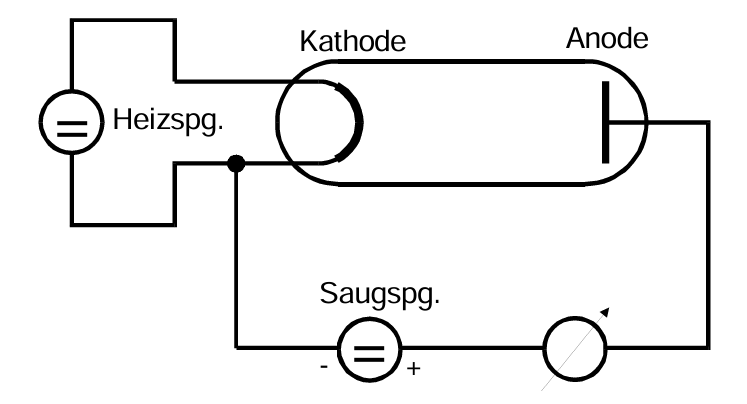
\includegraphics[width=0.65\textwidth]{content/Schaltung.png}
            \caption{Schaltung einer Hochvakuumdiode und Aufbau des Experiments \cite{Versuchsanleitung_v504}.}
        \end{center}
    \end{wrapfigure}
    Der Versuchsaufbau wird nach dem Grundsatz der nebenstehenden Schaltung aufgebaut. An der Glühkathode 
    befindet sich so eine Heizspannung. Die Anode ist mit der Kathode über eine Saugspannung verbunden. 
    Außerdem ist ein Strommessgerät in Reihe zur Anode geschaltet, welches den Saugstrom misst. So kann 
    die Kennlinie der Hochvakuumdiode aufgenommen werden. Die Glühkathode besteht aus einem Wolframdraht. \\
\end{minipage}
\noindent Da der Anlaufstrom sehr klein ist, wird für die Aufzeichnung des Anlaufstroms ein empfindlicheres 
Strommessgerät verwendet als für den restlichen Teil der Kennlinie.
Zur Aufzeichnung des Anlaufstroms wird außerdem ein Gegenfeld aufgebaut, sodass negative Spannungen 
realisiert werden und immer weniger Elektronen die Anode erreichen. 

\newpage

\section{Messwerte}
\label{sec:Messwerte}

Die für die Anlaufspannung entstehenden Messwerte sind in der folgenden Tabelle aufgeführt. 
Die Heizspannung beträgt hierbei \qty{5 \pm 0.5}{\volt} bei einem Heizstrom von \qty{2.4\pm 0.1}{\ampere}.
\begin{table}[H]
    \centering 
    \caption{Messung des Anlaufstromgebiets mithilfe der Gegenfeldmethode.}
    \begin{tblr}{
        colspec = {S[table-format=1.2] S[table-format=1.2]},
        row{1} = {guard, mode=math},
        }
        \toprule 
            \text{Saugspannung} \mathbin{/} \unit{\volt} & \text{Saugstrom} \mathbin{/} \unit{\nano\ampere} \\
        \midrule
        0.00    &   4.00    \\
        0.04    &   2.60    \\
        0.10    &   2.00    \\
        0.20    &   1.25    \\
        0.24    &   0.97    \\
        0.26    &   0.85    \\
        0.30    &   0.68    \\
        0.34    &   0.50    \\
        0.40    &   0.32    \\
        0.50    &   0.15    \\
        \bottomrule
    \end{tblr}
    \label{tab:Anlaufstromgebiet}
\end{table}

\noindent Die Vermessung der Kennlinie wird für fünf verschiedene Heizströme durchgeführt. 
Es gibt eine größere Wertedichte für den Bereich von \qty{0}{\volt} bis \qty{60}{\volt}, da die Skala 
des Strommessgeräts in diesem Abschnitt feiner ist und somit genauer gemessen werden kann.\\
\noindent Für die Heizspannung von \qty{4\pm 0.5}{\volt} und einem Heizstrom von \qty{2\pm 0.1}{\ampere} 
ergibt die Vermessung der Kennlinie die folgenden Werte.

\begin{table}[H]
    \centering 
    \caption{Messung der Kennlinie bei einer Heizspannung von \qty{4 \pm 0.5}{\volt} und \qty{2.0\pm0.1}{\ampere}.}
    \begin{tblr}{
        colspec = {S[table-format=3.0] S[table-format=1.3]},
        row{1} = {guard, mode=math},
        }
        \toprule 
            \text{Saugspannung} \mathbin{/} \unit{\volt} & \text{Saugstrom} \mathbin{/} \unit{\milli\ampere} \\
        \midrule
        0       &   0.000   \\
        5       &   0.005   \\
        10      &   0.013   \\
        15      &   0.022   \\
        20      &   0.029   \\
        25      &   0.037   \\
        30      &   0.043   \\
        35      &   0.047   \\
        40      &   0.050   \\
        45      &   0.052   \\
        50      &   0.054   \\
        55      &   0.056   \\
        60      &   0.057   \\
        70      &   0.058   \\
        80      &   0.057   \\
        90      &   0.058   \\
        100     &   0.060   \\
        \bottomrule
    \end{tblr}
    \label{tab:Kennlinie2.0}
\end{table}

\noindent Die Messung wird für Heizströme von \qty{2.1\pm0.1}{\ampere} mit \qty{4\pm0.5}{\volt}, 
\qty{2.2\pm0.1}{\ampere} mit \qty{4.5\pm0.5}{\volt}, \qty{2.3\pm0.1}{\ampere} mit \qty{5\pm0.5}{\volt} und 
\qty{2.4\pm0.1}{\ampere} mit \qty{5\pm0.5}{\volt} wiederholt. Im Folgenden werden die zugehörigen Messwerte aufgeführt. 

\begin{table}[H]
    \caption{Messung der Kennlinie.}
    \label{tab:Kennlinie}
    \begin{minipage}[t]{0.5\textwidth}
        \vspace{0pt}
        \centering
        \subcaption{Heizstrom von \qty{2.1\pm0.1}{\ampere} bei \qty{4\pm0.5}{\volt}}
    \begin{tblr}{
    colspec = {S[table-format=3.0] S[table-format=1.3]},
    row{1} = {guard, mode = math} 
    }
    %subcaption 2.1A
    \toprule
    \text{Saugspannung} \mathbin{/} \unit{\volt} & \text{Saugstrom} \mathbin{/} \unit{\ampere} \\
    \midrule
    0       &   0.000   \\
    5       &   0.007   \\
    10      &   0.019   \\
    15      &   0.031   \\
    20      &   0.043   \\
    25      &   0.056   \\
    30      &   0.070   \\
    35      &   0.082   \\
    40      &   0.092   \\
    45      &   0.100   \\
    50      &   0.107   \\
    55      &   0.111   \\
    60      &   0.115   \\
    70      &   0.118   \\
    80      &   0.117   \\
    90      &   0.122   \\
    100     &   0.125   \\
    120     &   0.132   \\
    150     &   0.131   \\
    \end{tblr}
\end{minipage}\hfill
\begin{minipage}[t]{0.5\textwidth}
    \vspace{0pt}
    \centering
    \subcaption{Heizstrom von \qty{2.2\pm0.1}{\ampere} bei \qty{4.5\pm0.5}{\volt}}
    \begin{tblr}{
        colspec = {S[table-format=3.0] S[table-format=1.3]},
        row{1} = {guard, mode = math} 
        }
        %subcaption 2.2
        \toprule
        \text{Saugspannung} \mathbin{/} \unit{\volt} & \text{Saugstrom} \mathbin{/} \unit{\ampere} \\
        \midrule
        0       &   0.000   \\
        10      &   0.026   \\
        20      &   0.060   \\
        30      &   0.101   \\
        40      &   0.143   \\
        50      &   0.184   \\
        60      &   0.219   \\
        70      &   0.244   \\
        80      &   0.257   \\
        90      &   0.274   \\
        100     &   0.283   \\
        120     &   0.294   \\
        140     &   0.300   \\
        180     &   0.308   \\
        240     &   0.316   \\
        250     &   0.318   \\
        \end{tblr}
    \end{minipage}\hfill
\end{table}
%

%
\begin{table}[H]
    \caption{Messung der Kennlinie.}
    \label{tab:Kennlinie}
    \begin{minipage}[t]{0.5\textwidth}
        \vspace{0pt}
        \centering
        \subcaption{Heizstrom von \qty{2.3\pm0.1}{\ampere} bei \qty{5\pm0.5}{\volt}}
    \begin{tblr}{
    colspec = {S[table-format=3.0] S[table-format=1.3]},
    row{1} = {guard, mode = math} 
    }
    %subcaption 2.3A
    \toprule
    \text{Saugspannung} \mathbin{/} \unit{\volt} & \text{Saugstrom} \mathbin{/} \unit{\ampere} \\
    \midrule
    0       &   0.000\\
    10      &   0.030\\
    20      &   0.073\\
    30      &   0.126\\
    40      &   0.181\\
    50      &   0.238\\
    60      &   0.300\\
    70      &   0.354\\
    80      &   0.409\\
    90      &   0.464\\
    100     &   0.508\\
    120     &   0.572\\
    140     &   0.606\\
    160     &   0.627\\
    180     &   0.639\\
    200     &   0.648\\
    220     &   0.655\\
    240     &   0.661\\
    250     &   0.664\\
    \end{tblr}
\end{minipage}\hfill
\begin{minipage}[t]{0.5\textwidth}
    \vspace{0pt}
    \centering
    \subcaption{Heizstrom von \qty{2.4\pm0.1}{\ampere} bei \qty{5\pm0.5}{\volt}}
    \begin{tblr}{
        colspec = {S[table-format=3.0] S[table-format=1.3]},
        row{1} = {guard, mode = math} 
        }
        %subcaption 2.4
        \toprule
        \text{Saugspannung} \mathbin{/} \unit{\volt} & \text{Saugstrom} \mathbin{/} \unit{\ampere} \\
        \midrule
        0       &   0.000\\
        3       &   0.006\\
        6       &   0.014\\
        9       &   0.023\\
        12      &   0.033\\
        15      &   0.044\\
        18      &   0.058\\
        21      &   0.073\\
        24      &   0.090\\
        27      &   0.100\\
        30      &   0.123\\
        33      &   0.144\\
        36      &   0.163\\
        39      &   0.181\\
        42      &   0.202\\
        45      &   0.223\\
        48      &   0.246\\
        51      &   0.270\\
        54      &   0.295\\
        57      &   0.322\\
        60      &   0.349\\
        70      &   0.435\\
        80      &   0.521\\
        90      &   0.607\\
        100     &   0.681\\
        120     &   0.835\\
        140     &   0.959\\
        160     &   1.068\\
        180     &   1.146\\
        200     &   1.201\\
        220     &   1.238\\
        240     &   1.263\\
        250     &   1.272\\
        \end{tblr}
    \end{minipage}\hfill
\end{table}



%\end{document}

